\section{Auswertung}
Alle Ausgleichsrechnungen werden mit dem Paket \texttt{scipy.optimize.curve\_fit}  aus \texttt{Python 3.7.3} durchgeführt.
Für Rechnungen mit fehlerbehafteten Größen wird das Paket \texttt{uncertainties} aus \texttt{Python 3.7.3} verwendet.

\subsection{Eichung des Magnetfeldes}
Im ersten Schritt der Auswertung werden die mit der Hallsonde aufgenommenen Werte für das
vorliegende Magnetfeld untersucht. Die gemessenen Daten der Stromstärke und die dazugehörige
Magnetfeldstärke sind in Tabelle \ref{Tab:Messwerte} aufgeführt.
\begin{table}[H]
    \centering
    \caption{Aufgenommene Werte der Magnetfeldstärke in Abhängigkeit der Stromstärke.}
    \label{tab:Messwerte}
    \begin{tabular}{cc}
      \toprule
      Stromstärke I\, / \, $\si{\ampere}$ & B-Feld \, / \, $\si{\milli\tesla}$  \\
      \midrule
      0 &    5 \\
      1 &   78 \\
      2 &  138 \\
      3 &  208 \\
      4 &  262 \\
      5 &  330 \\
      6 &  388 \\
      7 &  440 \\
      8 &  503 \\
      9 &  558 \\
     10 &  610 \\
     11 &  659 \\
     12 &  740 \\
     13 &  830 \\
     14 &  915 \\
     15 & 1003 \\
     16 & 1076 \\
     17 & 1111 \\
     18 & 1142 \\
     19 & 1163 \\
     20 & 1183 \\
     21 & 1215 \\
      \bottomrule
  \end{tabular}
 \end{table} \noindent
 In Abbildung \ref{fig:Magnetfeld} sind die Messwerte zusammen mit einer linearen Ausgleichgerade der
 Form
 \begin{equation}
     B(I) = a \cdot I + b
 \end{equation} \noindent
 dargestellt.
 \begin{figure}[H]
     \centering
     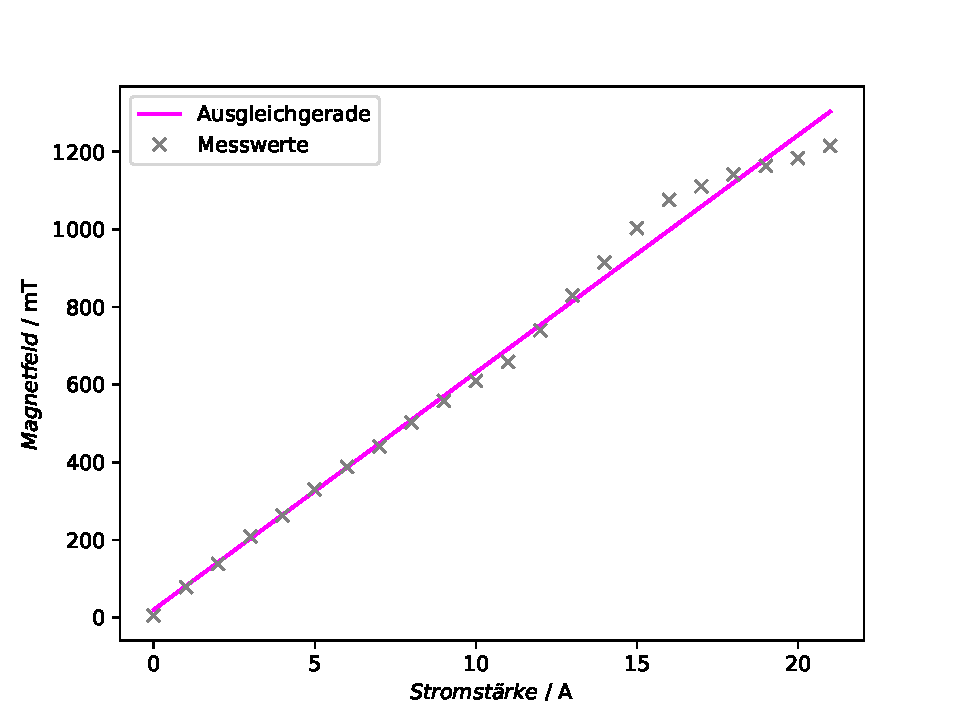
\includegraphics[width=0.8\textwidth]{Auswertung/Magnetfeld.pdf}
     \caption{Darstellung der aufgenommen Messwerte der Magnetfeldstärke in Abhängigkeit der Stromstärke zusammen
     mit einer linearen Ausgleichsgerade.}
     \label{fig:Magnetfeld}
 \end{figure} \noindent
 Die Regression liefert
 \begin{align}
     a &= \SI{61.08(129)}{\milli\tesla\per\ampere} \\
     b &= \SI{20.34(1581)}{\milli\tesla}
 \end{align} \noindent
 für die gesuchten Parameter.

 \subsection{Untersuchung der roten Spektrallinie}
 In Abbildung \ref{fig:rot} sind die aufgenommenen Interferenzbilder für die rote Spektrallinie
 mit einer Wellenlänge von $\lambda = \SI{643.8}{\nano\meter}$ dargestellt.
 \begin{figure}[H]
     \centering
     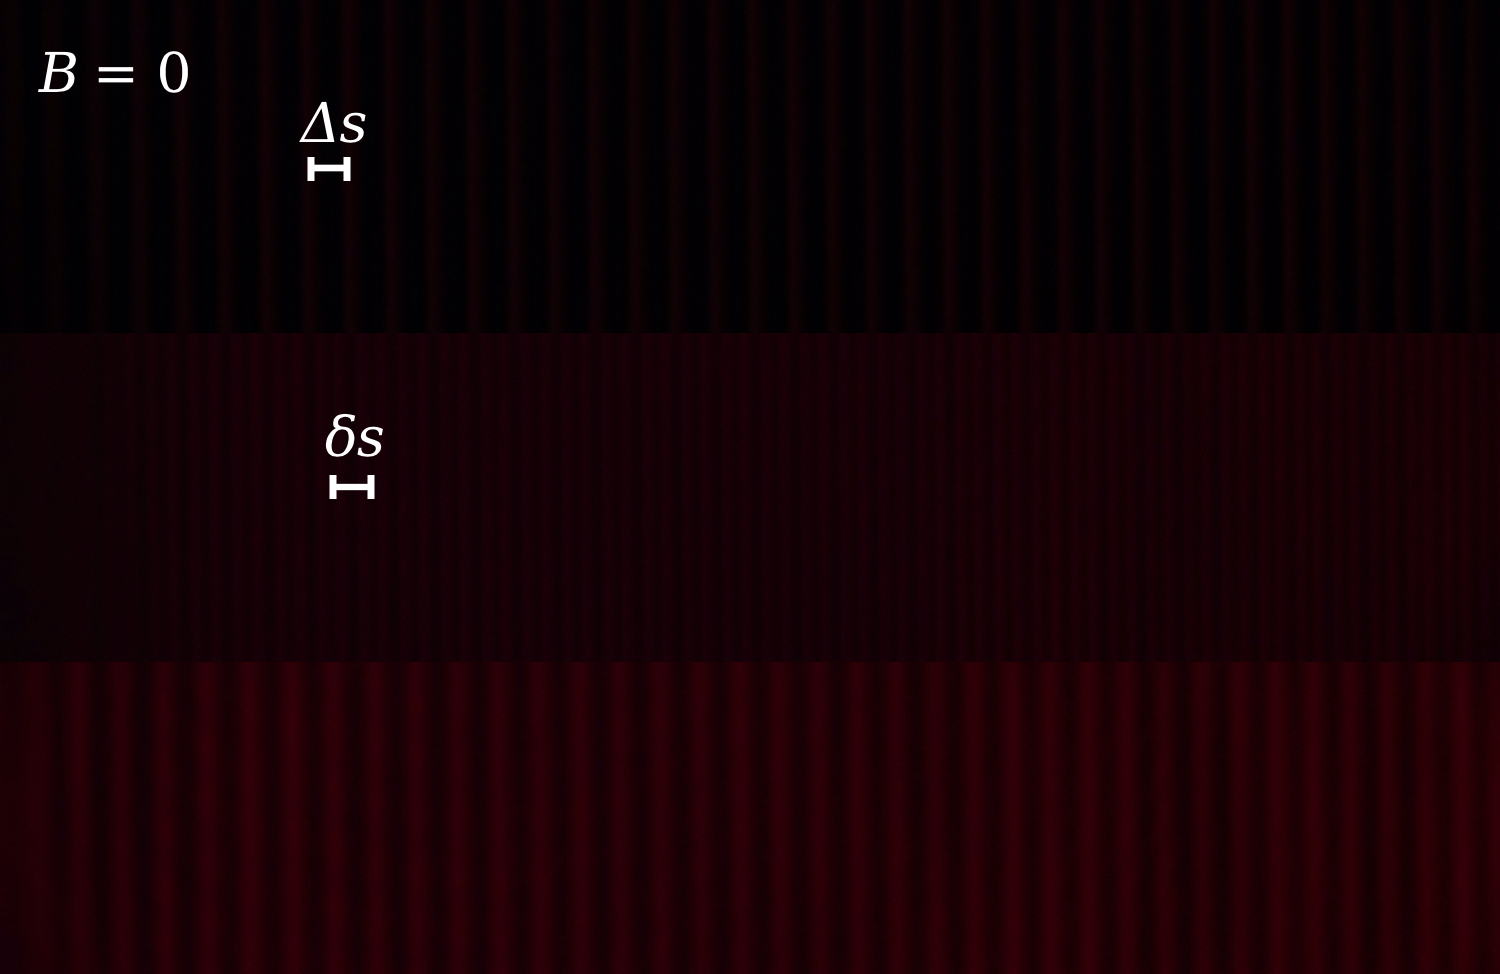
\includegraphics[width=0.8\textwidth]{images/zebraplot_rot.jpg}
     \caption{Darstellung von Ausschnitten aus den Aufnahmen der Interferenzmuster bei unterschiedlichen
     Einstellungen. Oben sind die Spektrallinien ohne Magnetfeldeinfluss zu sehen. Mittig und unten
     wird ein Magnetfeld von ca $\SI{692}{\milli\tesla}$ angelegt und die Polarisation von $\SI{0}{\degree}$ (Mitte)
     auf $\SI{90}{\degree}$ (Unten) umgestellt.}
     \label{fig:rot}
 \end{figure} \noindent
 Zu sehen sind die unterschiedlichen Interferenzen unter verschiedenen äußeren Einflüssen. Das obere der drei
 Bilder zeigt die Spektrallinie ohne den Einfluss eines Magnetfeldes und einer Polarisation. Der Ausschnitt in
 der Mitte zeigt die Spektrallinienaufspaltung bei einem Magnetfeld der Stärke $\SI{692}{\milli\tesla}$ und
 einer Polarisation von $\SI{0}{\degree}$. Dieser Übergang entspricht dem $\sigma$-Übergang. Das untere
 Bild zeigt dementsprechend die $\pi$-Übergange. Dabei liegt ebenfalls ein Magnetfeld von $\SI{692}{\milli\tesla}$
 an, die Polarisation entspricht jedoch $\SI{90}{\degree}$. Bei diesem Übergang kommt es jedoch zu keiner
 Auspaltung, da hier $\Delta m = 0$ vorliegt und somit nach Gleichung \ref{egn:E_normal} keine Energiedifferenz
 entsteht. \\
 Die Abstände zwischen den Maxima werden mithilfe eines Bildbearbeitungsprogammes als ein Pixelanzahl bestimmt.
 Die auf diese Weise bestimmten Werte sind in Tabelle \ref{tab:rot} zusammen mit den entsprechend berechneten
 Wellenlängenverschiebungen, die mit Formel \ref{eqn:WV} berechnet werden, aufgeführt.
 \begin{table}[H]
    \centering
    \caption{Die für die Maxima bestimmten Pixelabstände und die darausberechneten Wellenlängenverschiebungen für
    die ersten 10 Ordnungen.}
    \label{tab:rot}
    \begin{tabular}{c|ccc}
      \toprule
      Ordnung & $\Delta s_\text{rot}$ \, / \, \# Pixel & $\delta s_\text{rot}$ \, / \, \# Pixel & $\delta \lambda_\mathrm{rot,\sigma} \, / \, \si{\pico\meter}$ \\
      \midrule
       1 & 33 & 16 & 11,88 \pm 2,48\\
       2 & 35 & 17 & 11,90 \pm 2,33\\
       3 & 34 & 16 & 11,53 \pm 2,39\\
       4 & 32 & 15 & 11,48 \pm 2,54\\
       5 & 34 & 15 & 10,81 \pm 2,36\\
       6 & 33 & 16 & 11,88 \pm 2,48\\
       7 & 31 & 16 & 12,65 \pm 2,67\\
       8 & 33 & 18 & 13,36 \pm 2,54\\
       9 & 34 & 18 & 12,97 \pm 2,45\\
      10 & 31 & 15 & 11,85 \pm 2,63\\
      \bottomrule
  \end{tabular}
 \end{table} \noindent
 Da die Abstände der Maxima mit dem Auge abgeschätzt werden, werden sie mit einer Unsicherheit von 3 Pixeln
 betrachtet. Damit ergibt sich für den Gesamtfehler auf die Wellenlängenverschiebung nach Gauß
 \begin{equation}
     \Delta (\delta \lambda) = \frac{1}{2} \Delta \lambda \sqrt{\frac{1}{\Delta s^2} \cdot \Delta (\delta s)^2 + \left(\frac{\delta s}{(\Delta s)^2}\right)^2 \cdot \Delta (\Delta s)^2}.
 \end{equation} \noindent
 Aus den berechneten Werten für die Wellenlängenverschiebung ergibt sich durch Berechnung des Mittelwerts
 \begin{equation}
     \delta \lambda = \SI{12.03(79)}{\pico\meter}.
 \end{equation}


 \subsection{Untersuchung der blauen Spektrallinie}
 Analog dazu sind in Abbildung \ref{fig:blau} Auschnitte aus den Aufnahmen bei der Untersuchung der blauen
 Spektrallinie mit einer Wellenlänge von $\SI{450}{\nano\meter}$.
 \begin{figure}[H]
     \centering
     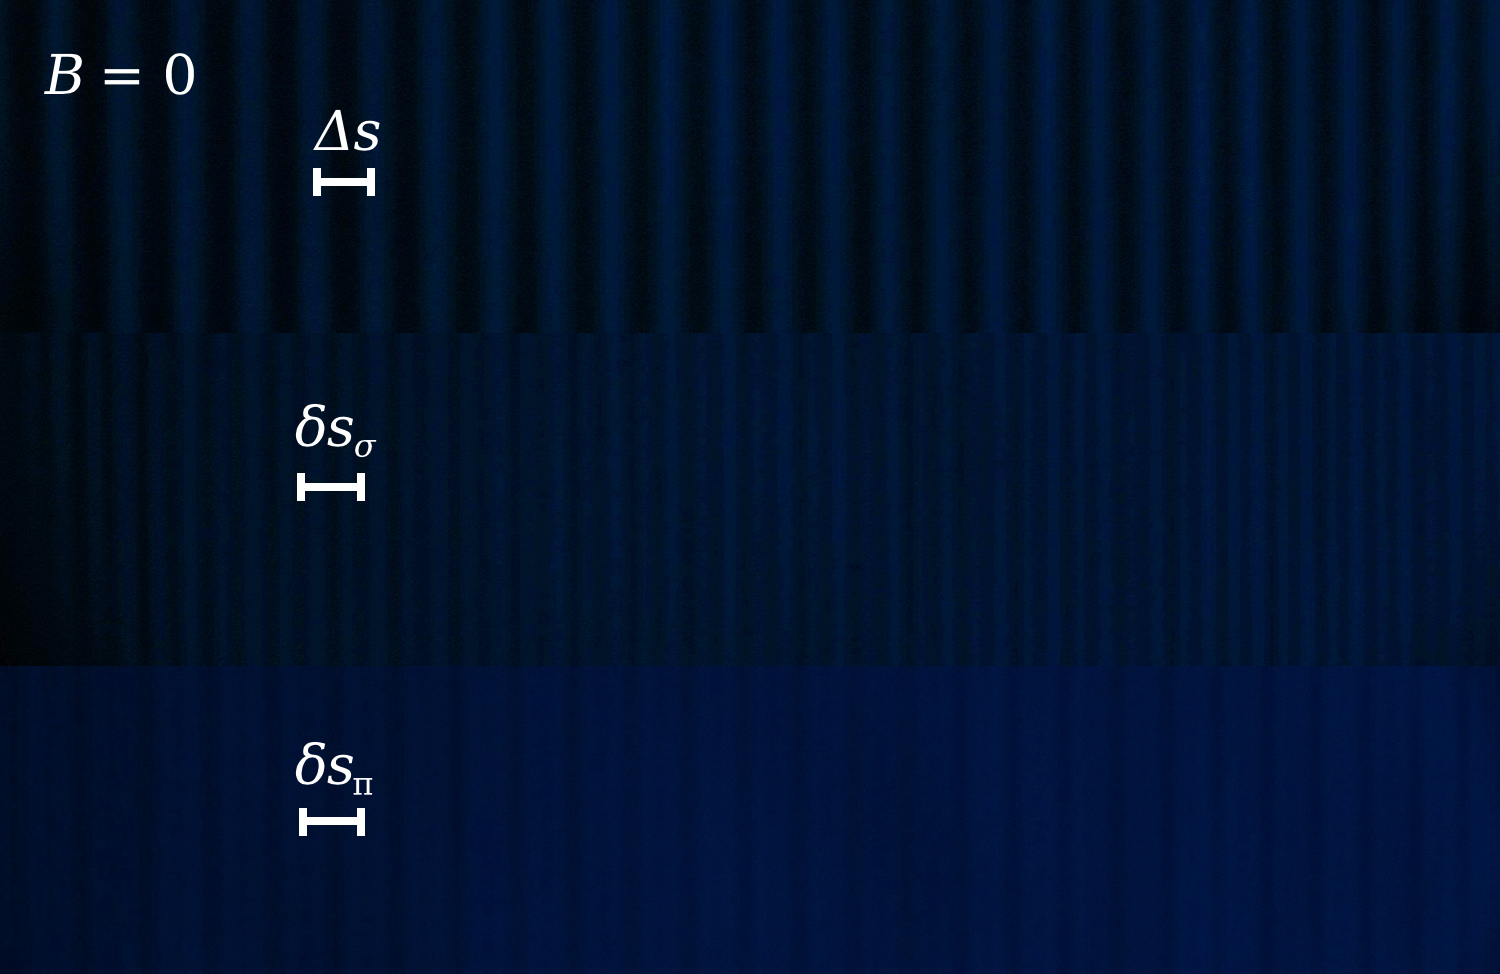
\includegraphics[width=0.8\textwidth]{images/zebraplot_blau.jpg}
     \caption{Darstellung von Ausschnitten aus den Aufnahmen der Interferenzmuster bei unterschiedlichen
     Einstellungen. Oben sind die Spektrallinien ohne Magnetfeldeinfluss zu sehen. In dem mittleren Bild 
     liegt ein Magnetfeld von $\SI{372}{\milli\tesla}$ und eine Polarisation von $\SI{0}{\degree}$ vor. Im 
     unteren Bild wird die Polarisation auf $\SI{90}{\degree}$ mit $\SI{1181}{\milli\tesla}$ eingestellt.}
     \label{fig:blau}
 \end{figure} \noindent
 Da in diesem Fall der anormale Zeeman-Effekt vorliegt, sind sowohl bei einer Polarisation von
 $\SI{0}{\degree}$ ($\sigma$-Übergang) als auch bei einer Polarisation von $\SI{90}{\degree}$ ($\pi$-Übergang)
 Wellenlängenverschiebungen zu erkennen. Daher werden für beide Übergänge separat die Interferenzabstände
 und die daraus resultierende Wellenlängenverschiebungen bestimmt. Diese sind in Tabelle \ref{tab:blau}
 aufgeführt.
 \begin{table}[H]
    \small
    \centering
    \caption{Die für die Maxima bestimmten Pixelabstände und die darausberechneten Wellenlängenverschiebungen für
    die ersten 10 Ordnungen.}
    \label{tab:blau}
    \begin{tabular}{cc|cc|cc}
      \toprule
      Ordnung & $\Delta s_\text{blau}$ \, / \, \#Pixel & $\delta s_\mathrm{blau, \sigma}$ \, / \, \#Pixel & $\delta \lambda_\mathrm{blau,\sigma} \, / \, \si{\pico\meter}$
      & $\delta s_\mathrm{blau, \pi}$ \, / \, \#Pixel & $\delta \lambda_\mathrm{blau,\pi} \, / \, \si{\pico\meter}$  \\
      \midrule
       1 & 47 & 26 & 7,47 \pm 1,64 & 16 & 4,60 \pm 1,52\\
       2 & 48 & 26 & 7,31 \pm 1,60 & 19 & 5,34 \pm 1,56\\
       3 & 50 & 24 & 6,48 \pm 1,50 & 20 & 5,40 \pm 1,45\\
       4 & 47 & 25 & 7,18 \pm 1,63 & 19 & 5,46 \pm 1,55\\
       5 & 45 & 23 & 6,90 \pm 1,68 & 19 & 5,70 \pm 1,63\\
       6 & 46 & 26 & 7.63 \pm 1,69 & 17 & 4,99 \pm 1,56\\
       7 & 45 & 23 & 6,90 \pm 1,68 & 21 & 6,30 \pm 1,66\\
       8 & 43 & 25 & 7,85 \pm 1,82 & 16 & 5,02 \pm 1,67\\
       9 & 44 & 22 & 6,75 \pm 1,72 & 20 & 6,14 \pm 1,69\\
      10 & 42 & 23 & 7,39 \pm 1,83 & 19 & 6,11 \pm 1,76\\
      \bottomrule
  \end{tabular}
 \end{table} \noindent
 Die Berechnugen der Wellenlängenverschiebungen, sowie die Fehler werden analog zur Rechnung der
 roten Spektrallinien bestimmt. Da die Maxima bei Betrachtung der blauen Spektrallinien etwas schwieriger
 ist als zuvor , wird hierbei eine Unsicherheit von 5 Pixeln angenommen.
 Eine Mittelung der zuvor berechneten Wellenlängen ergibt
 \begin{equation}
    \delta \lambda_\mathrm{blau,\sigma} = \SI{7,19(53)}{\pico\meter}
 \end{equation}
 und
 \begin{equation}
    \delta \lambda_\mathrm{blau,\pi} = \SI{5,51(51)}{\pico\meter}.
 \end{equation}

 \subsection{Bestimmung der Landé-Faktoren}
 Mithilfe der zuvor berechneten Wellenlängenverschiebungen können im Zusammenhang mit der Magnetfeldeichung
 die Landé-Faktoren der einzelnen Übergange bestimmt werden. Da sich die Photonenenergie nicht linear mit der
 Wellenlänge verhält, wird zunächst der Zusammenhang
 \begin{equation}
     \frac{\delta E}{\delta \lambda} = \frac{\delta}{\delta \lambda} \frac{hc}{\lambda} = -\frac{hc}{\lambda}
 \end{equation} \noindent
 hergestellt. Daraus folgt
 \begin{equation}
     |\delta E| = \frac{hc}{\lambda} |\delta \lambda|.
 \label{eqn:1}
 \end{equation} \noindent
 Somit gilt durch Einsetzen der Gleichung \ref{eqn:1} in Formel \ref{eqn:}
 \begin{equation}
     g = |\delta \lambda_i| \frac{hc}{\mu_\text{B} B_i \lambda_i^2}
 \end{equation}
für den normalen Zeeman-Effekt, sowie
\begin{equation}
    g_ij = |\delta \lambda_i| \frac{hc}{\mu_\text{B} B_i \lambda_i^2}
\end{equation}
für den anormalen Zeeman-Effekt.
In Tabelle \ref{tab:lande} sind die verwendeten Stromstärken und die daraus errechneten Magnetfeldstärken
aufgeführt. Zusätzlich enthält sie die damit berechneten Landé-Faktoren für die drei untersuchten
Übergange der Cadmium-Lampe.
\begin{table}[H]
    \centering
    \caption{Aufführung der berechneten Landé-Faktoren zusammen mit den verwendeten Stromstärken bzw. Magnetfeldstärken und den Wellenlängenverschiebungen.}
    \label{tab:lande}
    \begin{tabular}{c c|cc|c|c}
      \toprule
      $\lambda \, / \, \si{\nano\meter}$ & Übergang & Stromstärke \, / \, $\si{\ampere}$ & Magnetfeld \, / \, $\si{\milli\tesla}$ & $\delta \lambda \, / \, \si{\pico\meter}$ &  Landé-Faktor \\
      \midrule
        643,8 & $\sigma$ & 11,00 &  692,22 \pm 21,24 & 12,03 \pm 0,79 & 0,90 \pm 0,07\\
        480,0 & $\pi$    & 19,00 & 1180,86 \pm 29,17 & 5,51 \pm 0,51  & 0,43 \pm 0,04\\
        480,0 & $\sigma$ & 5,75  &  371,55 \pm 17,46 & 7,19 \pm 0,53  & 1,80 \pm 0,16\\
      \bottomrule
  \end{tabular}
 \end{table} \noindent
 Dabei berechnet sich der Fehler auf das Magnetfeld nach Gaußscher Fehlerfortpflanzung mit
 \begin{equation}
     \Delta B = \sqrt{(I\cdot \Delta a)^2 + \Delta b^2} .
 \end{equation}
 Ebenfalls über die Gaußsche Fehlerfortpflanzung gilt
 \begin{equation}
    \Delta g = \frac{hc}{\lambda^2 \mu_\text{B}} \sqrt{(\frac{1}{B} \cdot \Delta \delta \lambda)^2 + (\frac{\delta \lambda}{B^2}\cdot \Delta B)^2}
 \end{equation} \noindent
 für den Fehler auf die berechneten Landé-Faktoren.
